\documentclass[main.tex]{subfiles}

\begin{document}

\section{Branding}
\label{Branding}
We have started the process of creating a brand for our product by looking at books and articles on branding. The two most useful resources we have seen were \cite{basics_branding} and \cite{clifton_2009}. Based on the knowledge acquired, we have decided that our brand needs a name, a logo and a motto.

\subsection{Name and Logo}
In order to find a name and a logo that would represent us, we have conducted several brainstorming sessions where we have laid out the keywords that represent our product. Out of all the words we listed, two recurring categories appeared, which were `flourishing` and `data`. We then went on to find ways of representing those. At the end, we have decided on choosing `Thalia` as the name of the product, which is the name of a Greek muse often described as `the growing one`. We saw the association between our product and the Greek muse of growth as beneficial.

To create a logo to our liking, we have asked a young designer willing to create it Pro Bono for us. After a few iterations, we had two logos made from copyright free images, the smaller of which can be seen on \figurename{\ref{small_logo}}.

\begin{figure}[H]
    \centering
    
\includegraphics[scale=0.4]{00Branding/00Pictures/small_logo.png}
    \caption{Thalia Logo - Small}
    \label{small_logo}
\end{figure}

\subsection{Motto}

Based on our previous findings in \ref{reliability}, we have decided that our motto should be something that would reassure our customers that they have made the right choice. As a result, we have come up with a simple motto: `Thalia, the reliable Backtester`.


\subsection{Official colours} 

The idea of defining a set of official colours came from homogeneity. We strove for a uniform design both for our product and this report, so we believed it was a good way of ensuring this. Given our team's limited experience with design, we have decided to start by choosing the base colour of our palette. In order to be up to date with the latest design trends, we have sought to use something close to the colour of the year 2020 \cite{pantone}. Based on this colour, we have created three colour palettes by using a triadic colour scheme \cite{triadic}.

In the following figure, the final three colour schemes are presented. After some deliberation within the team and some feedback from a few outside people, we have decided to use the option labelled `Thalia`.

\begin{figure}[H]
    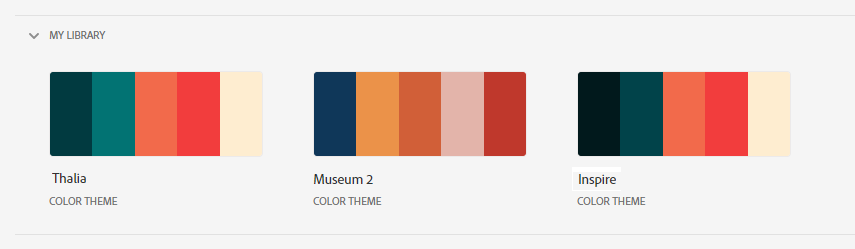
\includegraphics[width=\textwidth]{00Branding/00Pictures/color_schemes.png}
    \caption{Color Schemes}
\end{figure}

\end{document}    
